\section{Overview and System Contract}
\label{sec:overview}

\subsection{From file operations to storage choices}

To read \code{src/parser.py}, a client resolves its name, obtains the
visible inode and data mappings, and fetches the requested bytes. An
overwrite stores new payload and updates the file's metadata under the
selected durability contract. \sys separates three decisions along this
path: which state the task sees, how immutable metadata is retrieved, and
how payloads are divided into storage units
(Table~\ref{tab:mechanism-choices}). On the object path, $g$ denotes client
block size, $B$ denotes backend erasure-coding block size, and $q$ denotes
the physical verification/read quantum.

\begin{table*}[t]
\centering
\small
\begin{tabularx}{\textwidth}{@{}>{\raggedright\arraybackslash}p{3.0cm}YY@{}}
\toprule
Choice & Mechanism selected & Alternative retained\\
\midrule
View composition & Delta-based workspace: shared baseline plus private state & Ordinary volume with its own namespace and mappings\\
Immutable metadata & Packed Metadata: indexed records in bounded object-resident pages & Native catalog or KV representation\\
Object granularity & Configured client block size $g$; optional compatible backend $B/q$ choices & Fixed client geometry and backend default layout\\
\bottomrule
\end{tabularx}
\caption{Independent design decisions. Current mount paths admit specific
combinations, rather than eight interchangeable runtime modes.}
\label{tab:mechanism-choices}
\end{table*}

Composition rests on two interfaces. The lower reader resolves names,
attributes, and data locators under a fixed version identity; the data
path returns the referenced logical bytes under the object's persisted
layout. Changing the lower representation must preserve the first
contract, and choosing a storage layout must preserve the second.
Table~\ref{tab:mechanism-choices} retains alternatives at both boundaries.

\subsection{Pinning state and isolating changes}

Let $S$ identify a shared immutable baseline and $\Delta_i$ the private
writable state of workspace $i$. Its view is
\begin{equation}
  W_i = \operatorname{Resolve}(S,\Delta_i).
\end{equation}
Workspace creation pins $S$ so that subsequent lower queries refer to the
same version. The baseline exposes name, attribute, and data-location
queries through either a sealed native layer or a packed manifest.
It can cover a selected subtree without freezing an entire source volume.
Following a mutable latest pointer on each lookup would not preserve
this fixed starting state.

The isolation invariant is view-local mutation: an operation in $W_i$
leaves $S$ and another workspace's private state unchanged. Private names,
attributes, deletion markers, and data mappings determine which inherited
records remain visible. Section~\ref{sec:delta} specifies resolution and
the operation boundaries that preserve inode identity and prevent stale
bytes from reappearing. Process isolation and merging independent edits
require separate runtime or application protocols.

\subsection{Reading, writing, and publishing}

Figure~\ref{fig:overview} follows these parallel interfaces. An inherited
read obtains a locator from the chosen lower reader, then fetches its
payload range. An overwrite publishes a private mapping to new upper
bytes; other workspaces retain their references to $S$.

\begin{figure}[!t]
\centering
% Editable SVG with live text; regenerate with tools/draw_architecture_editable.py.
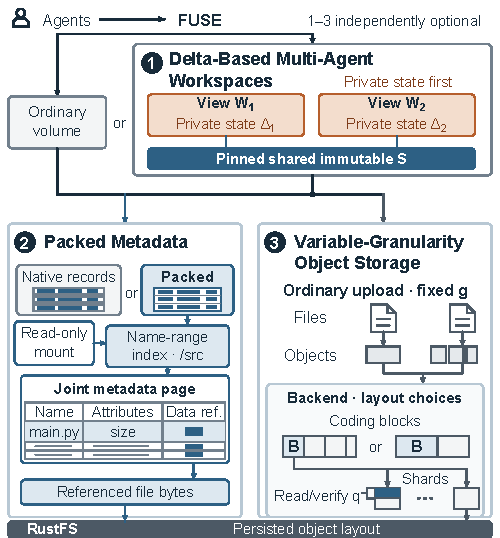
\includegraphics[width=\columnwidth]{figures/system-architecture-editable.pdf}

\caption{Independently optional mechanisms. Fixed $g$ alternatives split
the same aligned $10\MiB$ slice (raw MiB). Each block forms an object after
applicable formatting; $B$ sizes its erasure-coding blocks, while $q$ sizes
verification/read units within a shard. Backend geometry is schematic;
producer contracts and admission gates differ
(Section~\ref{sec:implementation}).}
\label{fig:overview}
\end{figure}

Writes introduce two visibility boundaries. A dirty buffer can serve
this client's reads before remote durability. Publishing a recoverable
version requires its referenced objects to satisfy the selected
persistence contract and its metadata to be validated.

Workspace and reader ownership must retain referenced metadata and
payloads until reclamation is safe. A published version may contain
application checkpoints; restoring process memory and open handles
remains the runtime's responsibility. Section~\ref{sec:implementation}
identifies the current mount and recovery paths.
